\subsubsection{pr04}
The obtained results were the following:
{
\renewcommand{\arraystretch}{2}
\begin{longtable}[h]{| c | c | c | c | c |}
    \hline
    \textbf{Failures} & \multicolumn{3}{c}{Time limit} & \\
    \hline
    \textbf{Search strategy} & \textbf{\textit{30 sec}} & \textbf{\textit{1 min}} & \textbf{\textit{2 min}} & \textbf{\textit{5 min}} \\
    \hline
    \endhead
    default search                                         & 238 &  3.590 &  6.941 &  30.405 \\
    \hline
    domWdeg, random                                        &  89 &  3.442 &  6.800 &  36.015 \\
    \hline
    domWdeg, random, Luby restart L=250                    &  76 &    76 &   759 &   4.460 \\
    \hline
    \textit{domWdeg, random, Luby restart L=250, LNS 85\%} &  76 &    76 &    76 &    107 \\
    \hline
    domWdeg, random, Luby restart L=250, LNS 15\%          &  76 &    76 &   755 &   6.566 \\
    \hline
    first fail, min                                        &  16 &    16 &  6.721 &  26.859 \\
    \hline
\end{longtable}
}
\begin{figure}[H]
    \centering
    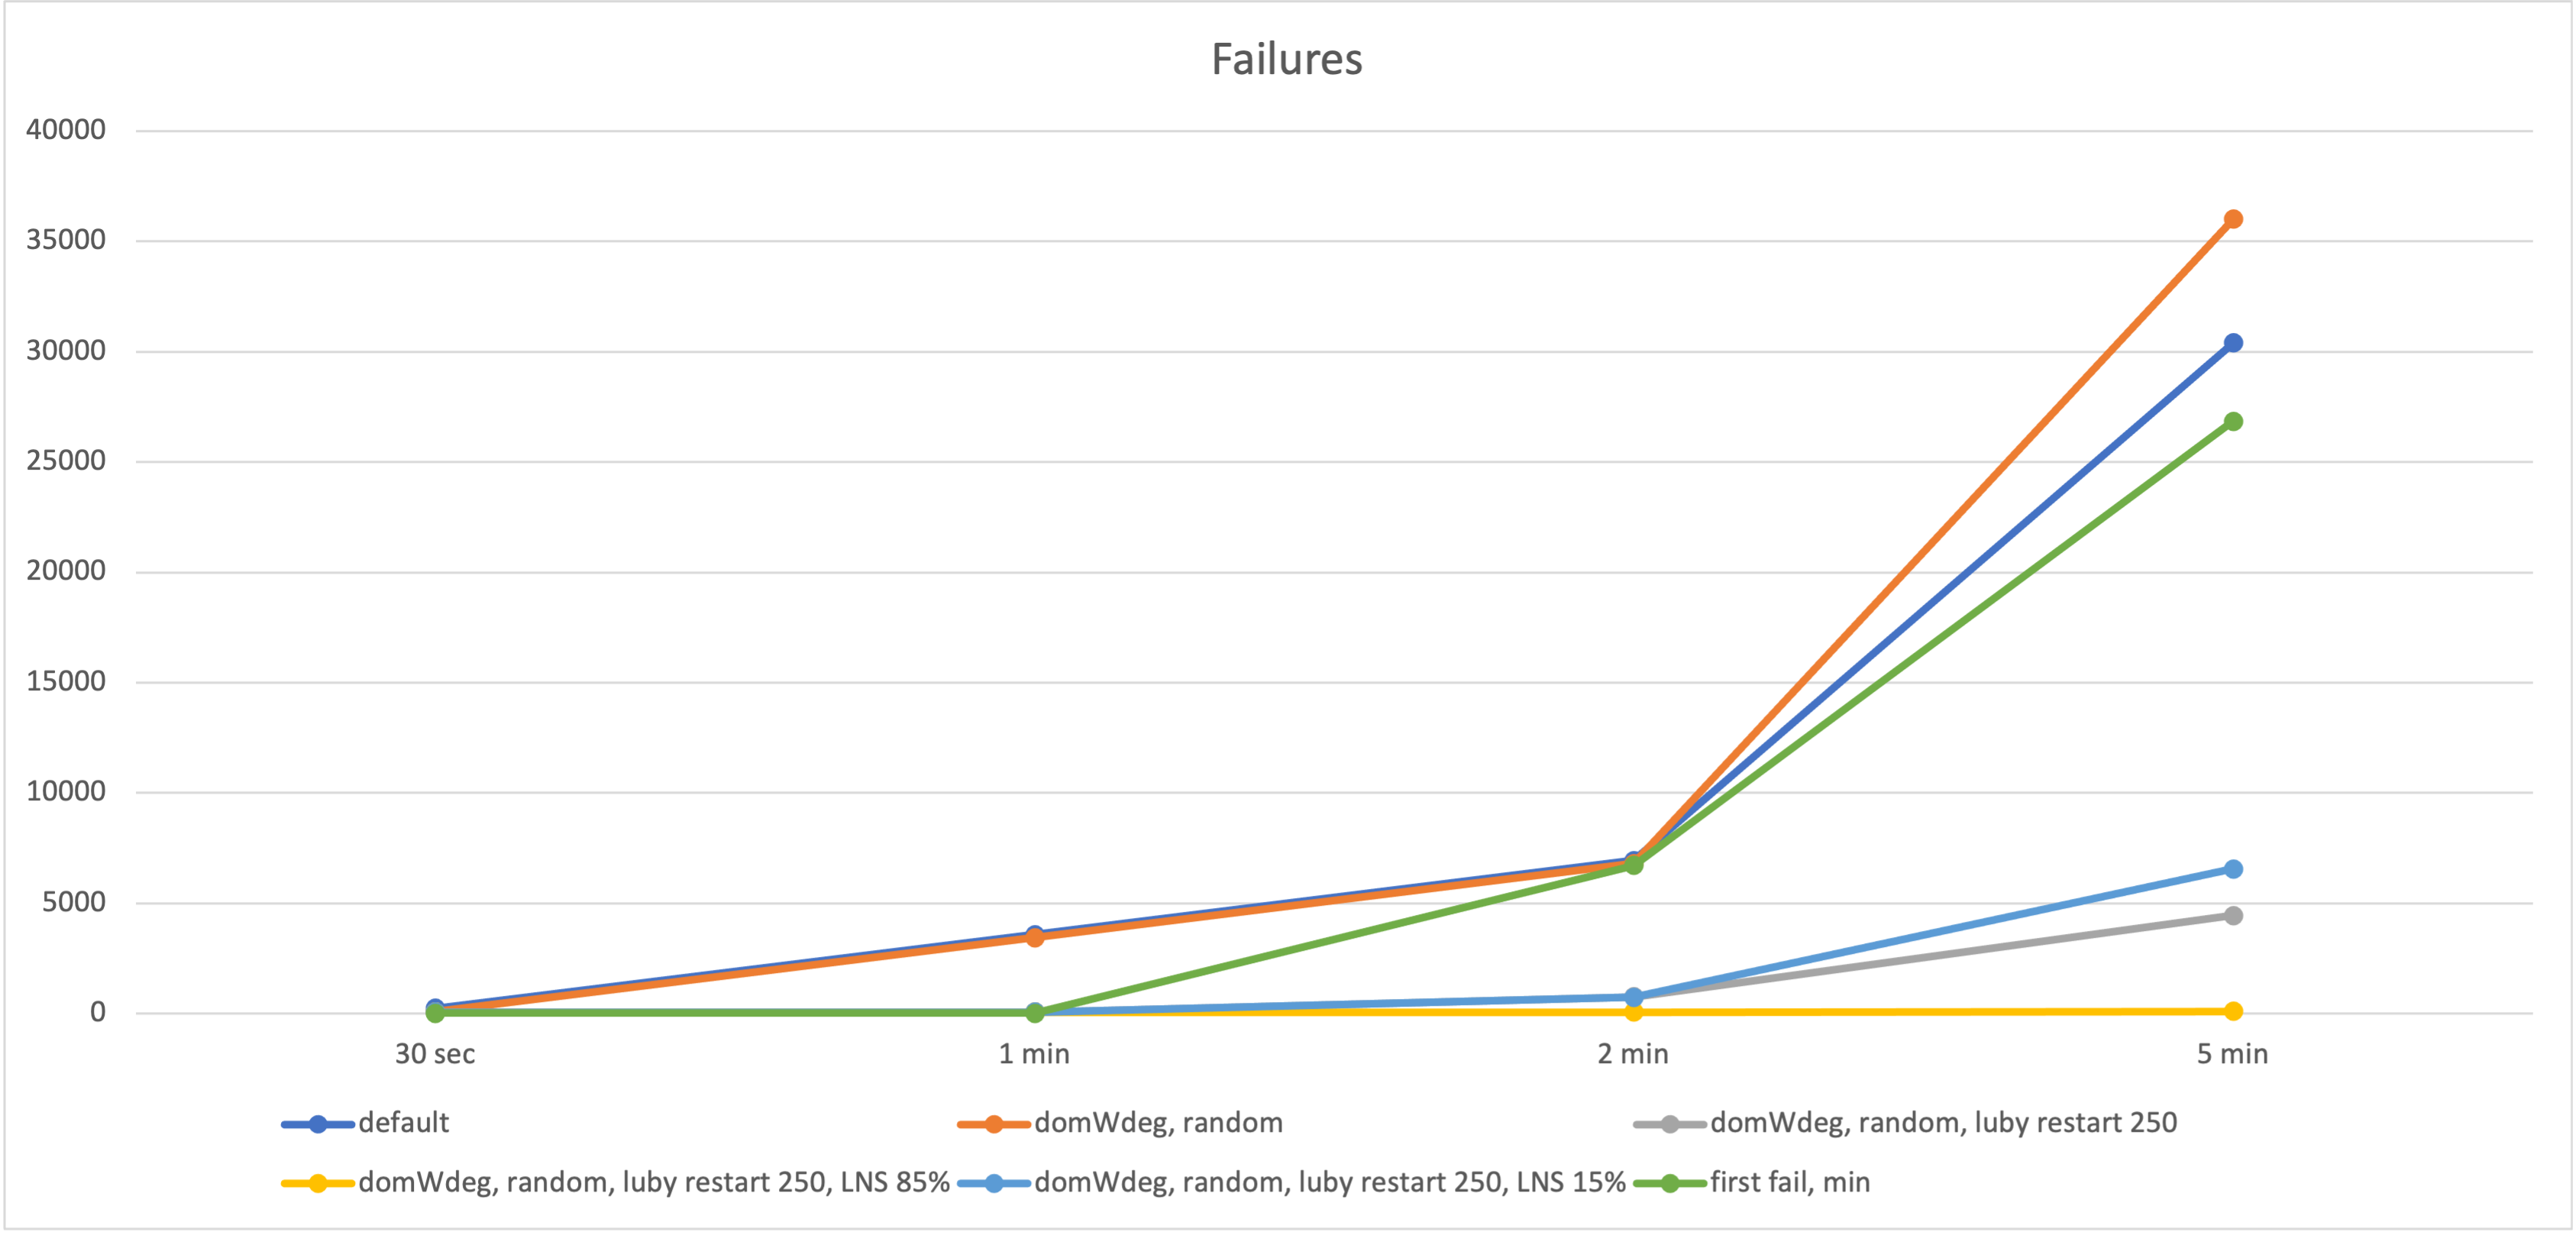
\includegraphics[width=1.0\columnwidth]{../graphs/pr04-failures.png}
    \caption{Failures graph for pr04.}
\end{figure}

{
\renewcommand{\arraystretch}{2}
\begin{longtable}[h]{| c | c | c | c | c |}
    \hline
    \textbf{Objective function} & \multicolumn{3}{c}{Time limit} & \\
    \hline
    \textbf{Search strategy} & \textbf{\textit{30 sec}} & \textbf{\textit{1 min}} & \textbf{\textit{2 min}} & \textbf{\textit{5 min}} \\
    \hline
    \endhead
    default search                                         &         - & 134.918.350 & 134.672.850 & 133.099.090 \\
    \hline
    domWdeg, random                                        &         - & 134.478.510 & 134.406.680 & 133.455.600 \\
    \hline
    domWdeg, random, Luby restart L=250                    &         - & 140.858.980 & 132.310.870 & 130.095.820 \\
    \hline
    domWdeg, random, Luby restart L=250, LNS 85\%          &         - & 140.858.980 & 140.346.770 & 135.802.770 \\
    \hline
    \textit{domWdeg, random, Luby restart L=250, LNS 15\%} &         - & 140.858.980 & 133.586.430 & 128.263.170 \\
    \hline
    first fail, min                                        &        - &         - & 138.358.940 & 137.061.510 \\
    \hline
\end{longtable}
}
\begin{figure}[H]
    \centering
    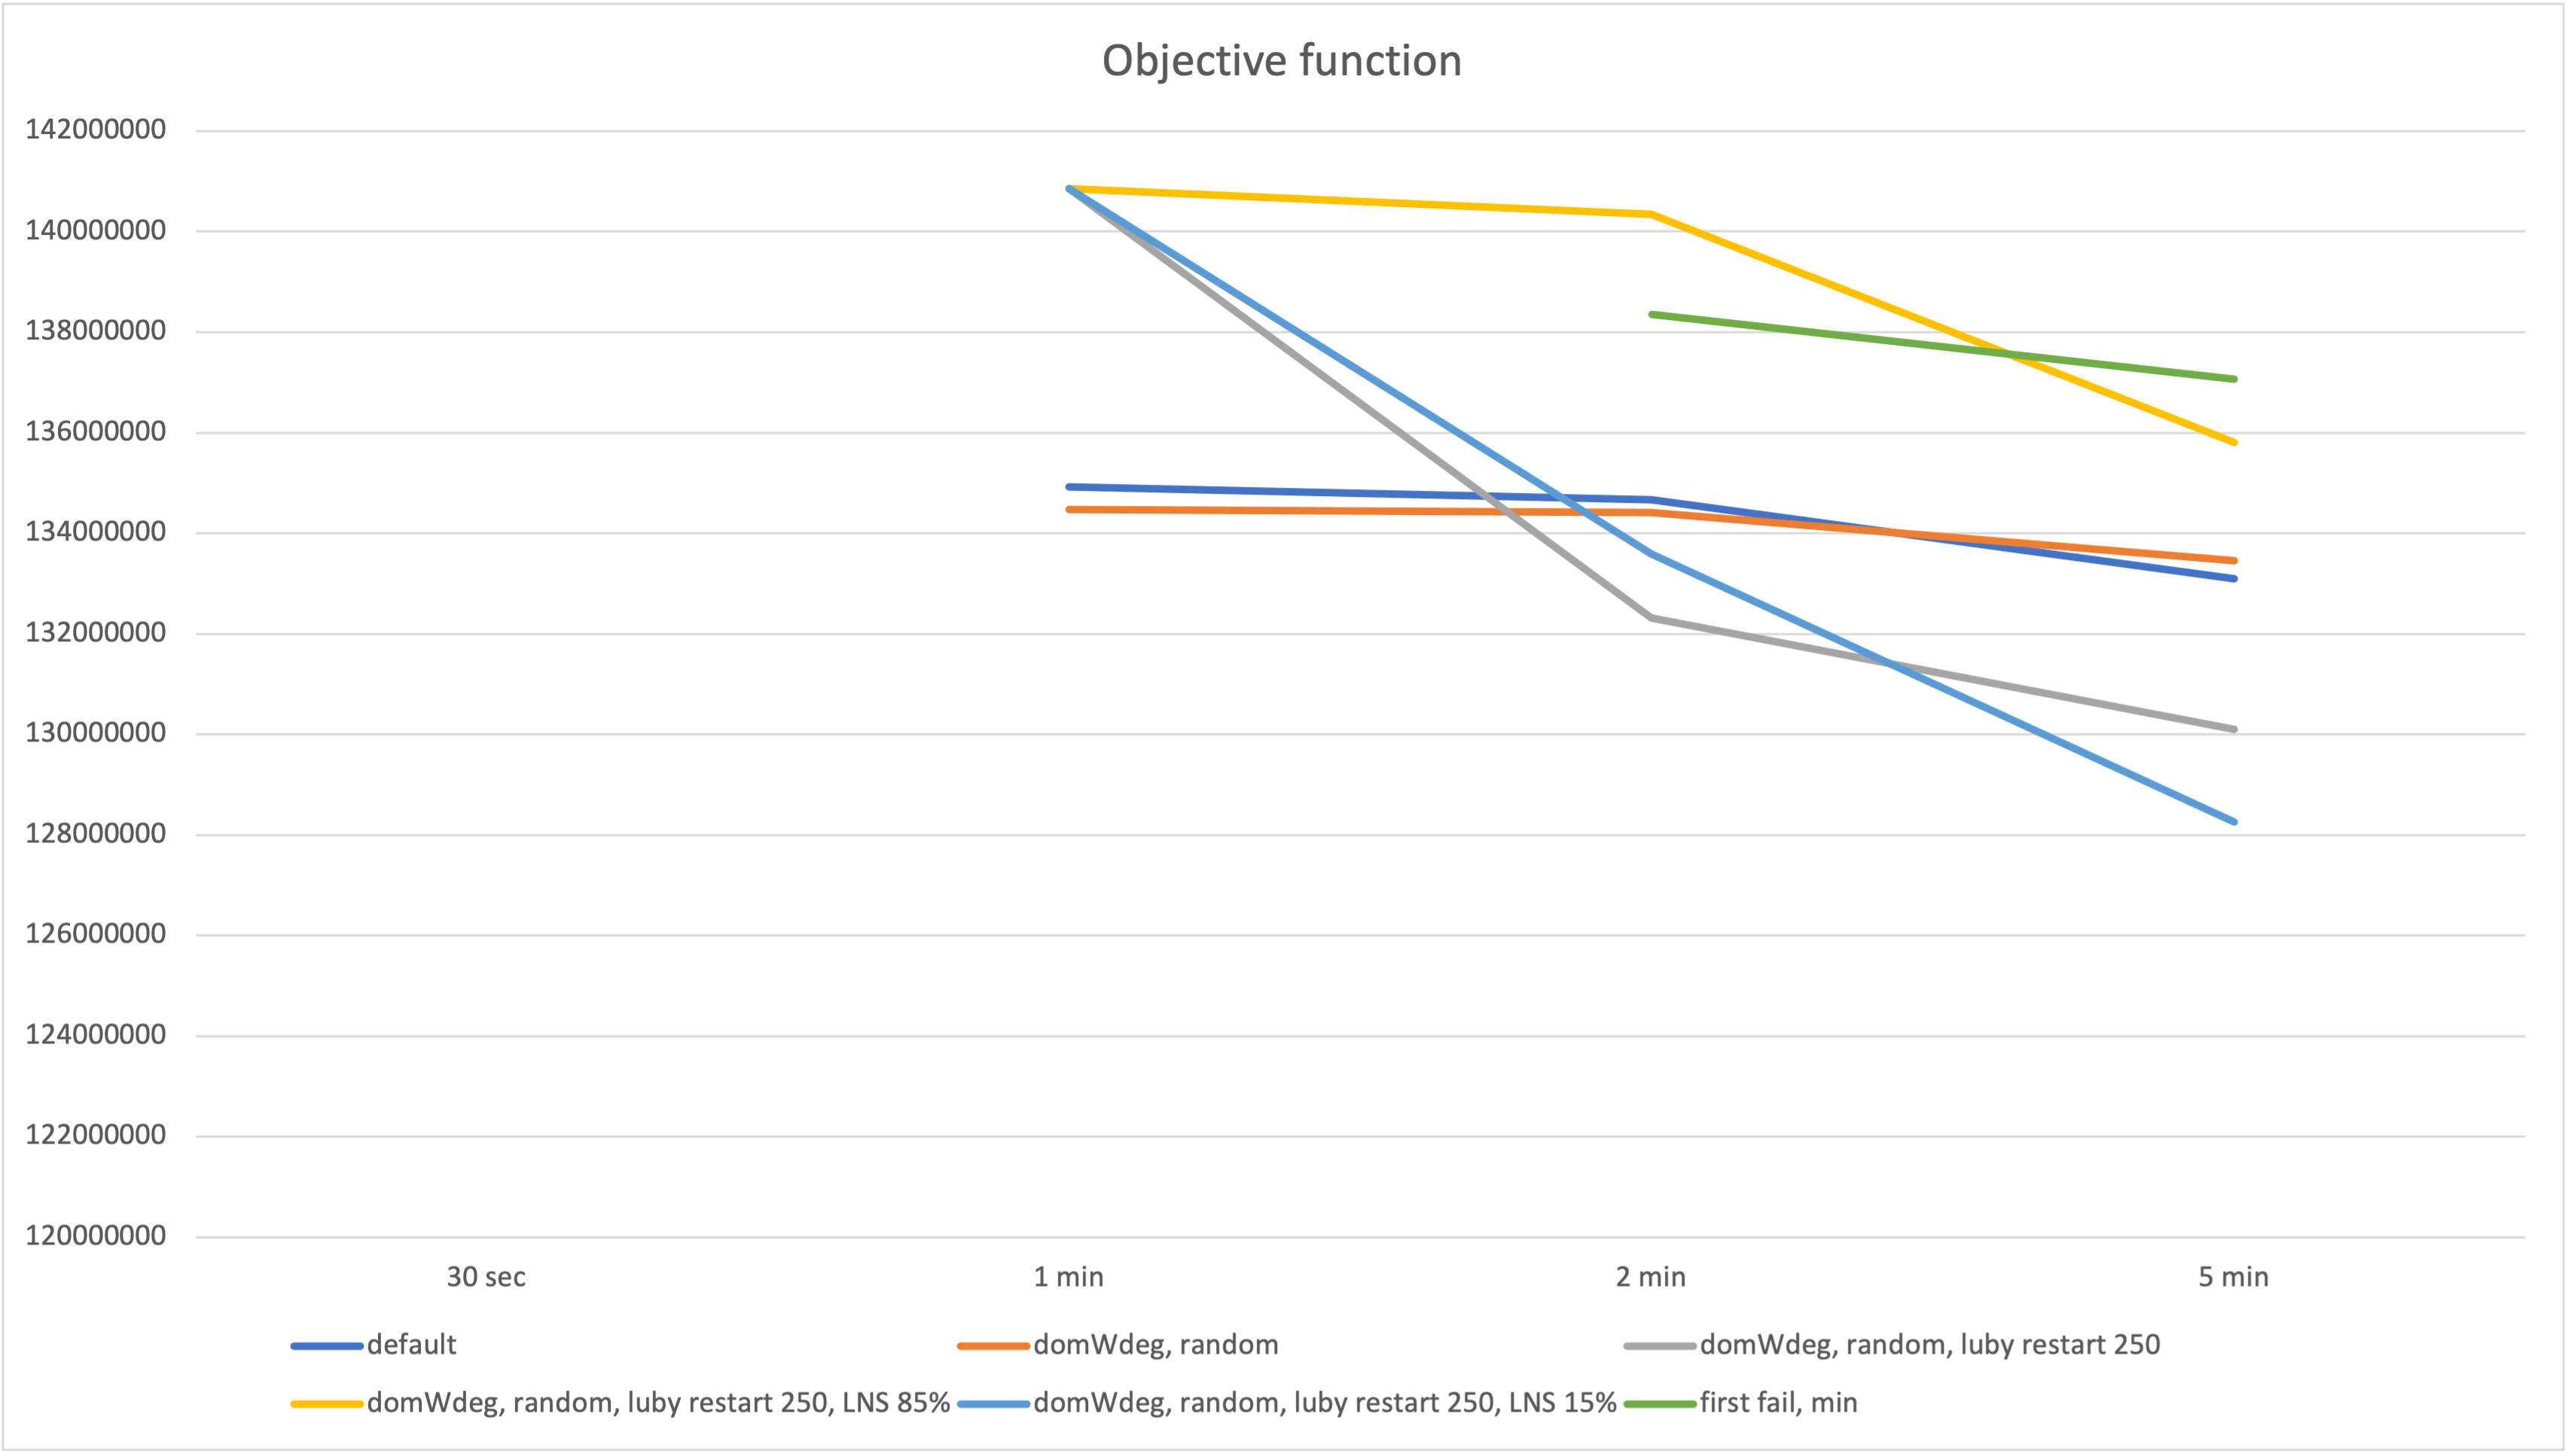
\includegraphics[width=1.0\columnwidth]{../graphs/pr04-objf.png}
    \caption{Objective functions graph for pr04.}
\end{figure}

{
\renewcommand{\arraystretch}{2}
\begin{longtable}[h]{| c | c | c | c |}
    \hline
    \textbf{Weights} & \textbf{Objective function} & \textbf{Total distance} & \textbf{Used vehicles} \\
    \hline
    \endhead
    $\alpha = 10, \beta = 0$ & 135.145.710 & 13.514.571 & 20 \\
    \hline
    $\alpha = 7, \beta = 3$  &  94.602.057 & 13.514.571 & 20 \\
    \hline
    $\alpha = 5, \beta = 5$  &  67.572.955 & 13.514.571 & 20 \\
    \hline
    $\alpha = 3, \beta = 7$  &  40.543.853 & 13.514.571 & 20 \\
    \hline
    $\alpha = 0, \beta = 10$ &         200 & 14.085.898 & 20 \\
    \hline
\end{longtable}
}
\begin{figure}[H]
    \centering
    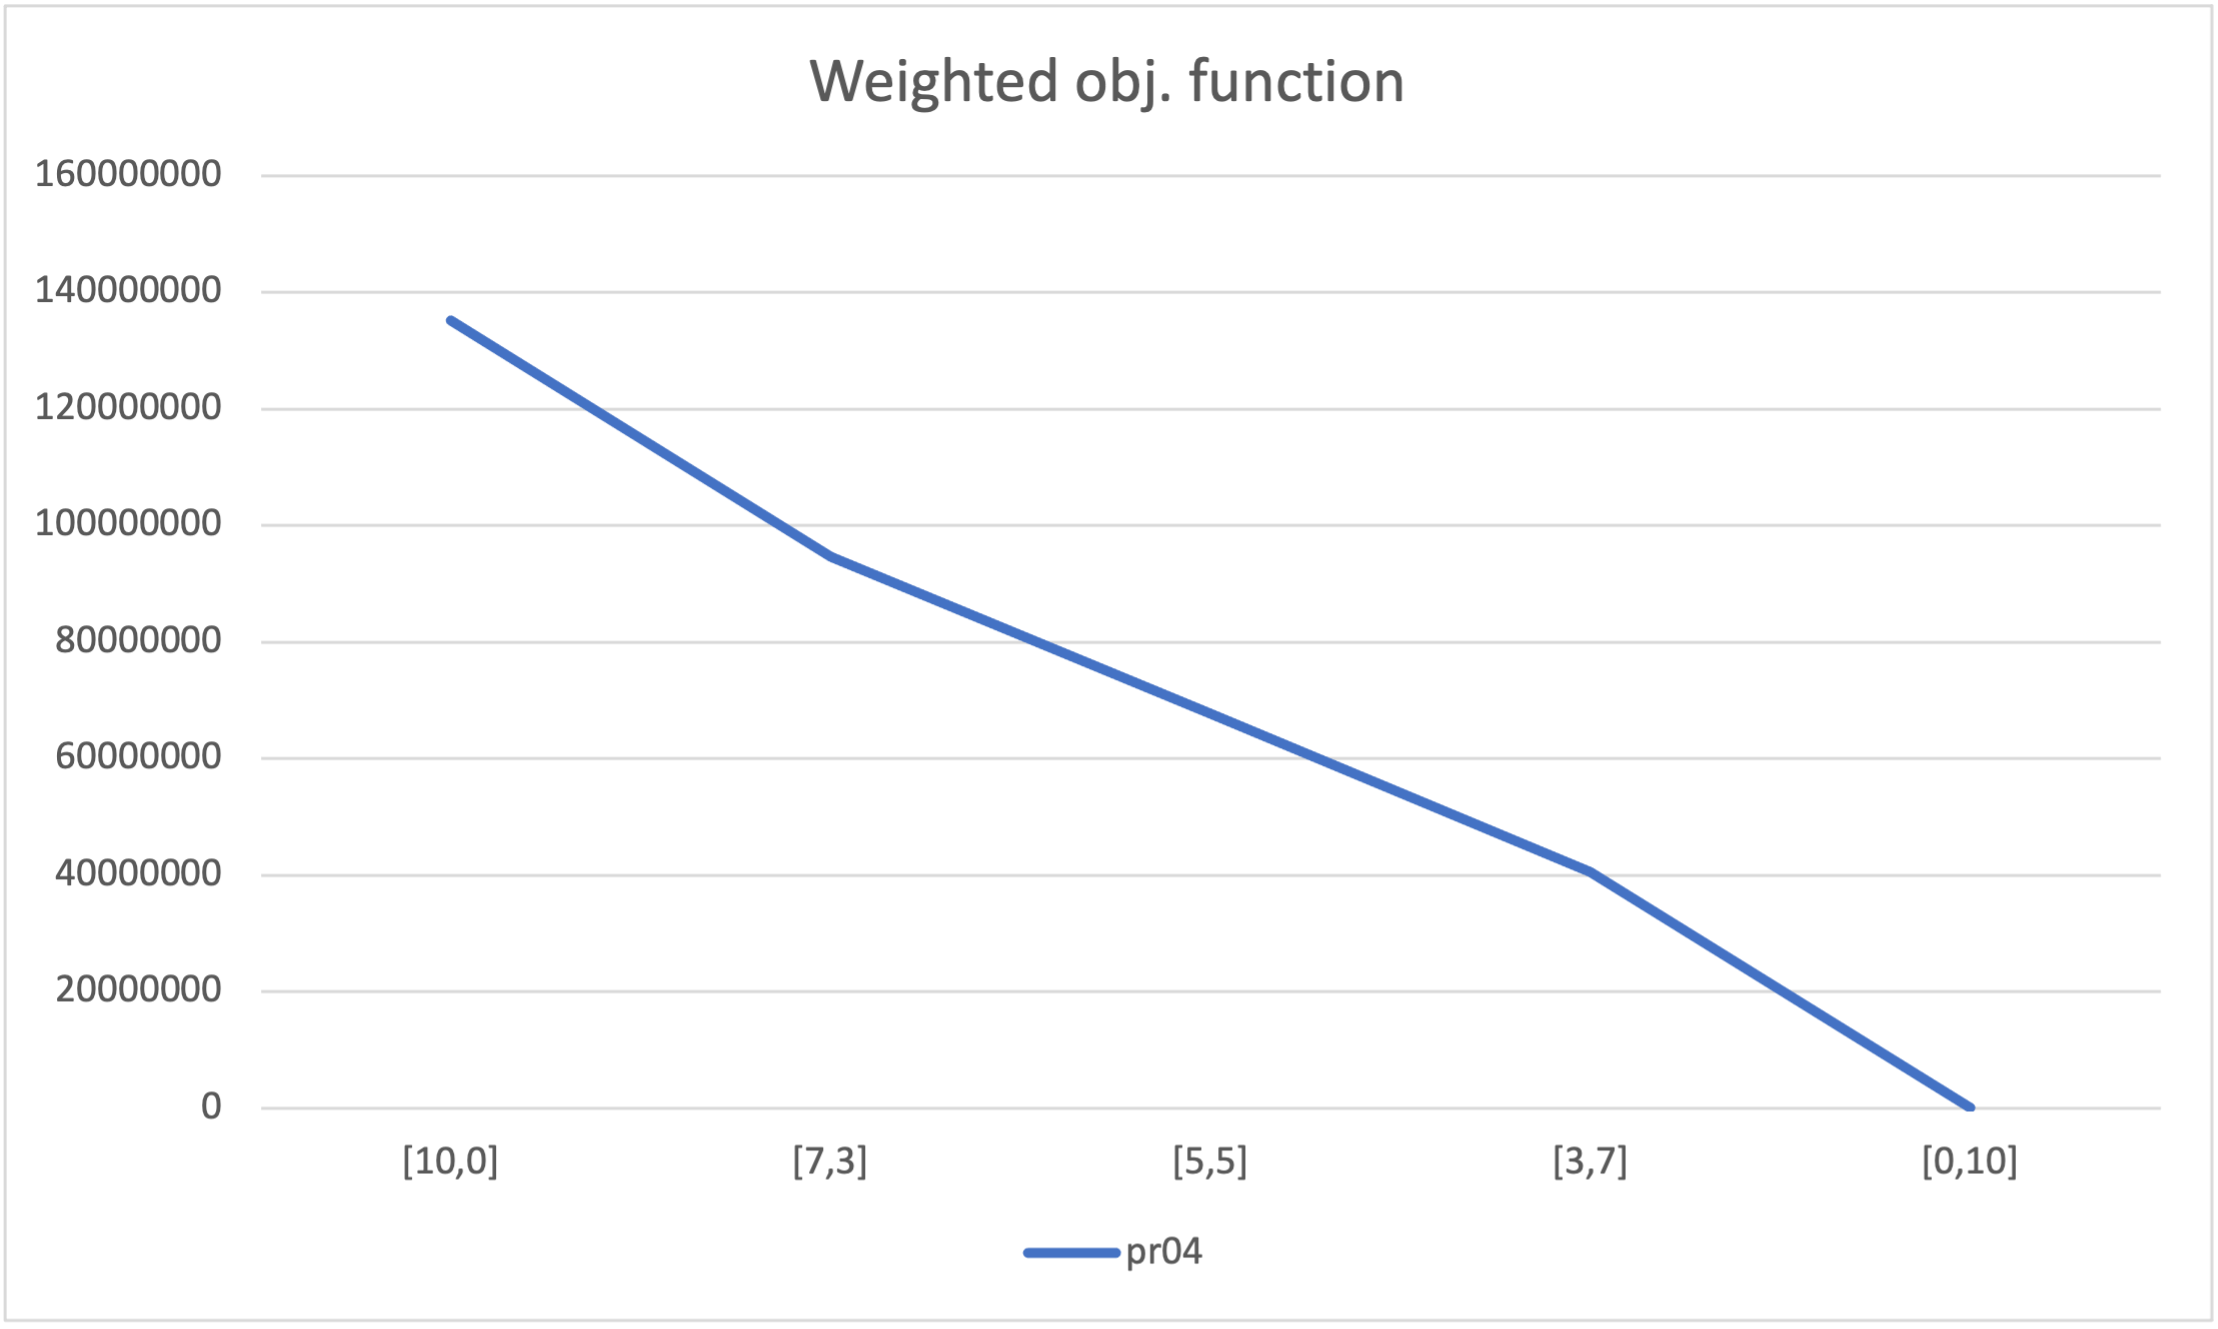
\includegraphics[height=0.25\textheight]{../graphs/pr04-wobjf.png}
    \caption{Weighted objective functions graph for pr04.}
\end{figure}

\begin{figure}[H]
    \centering
    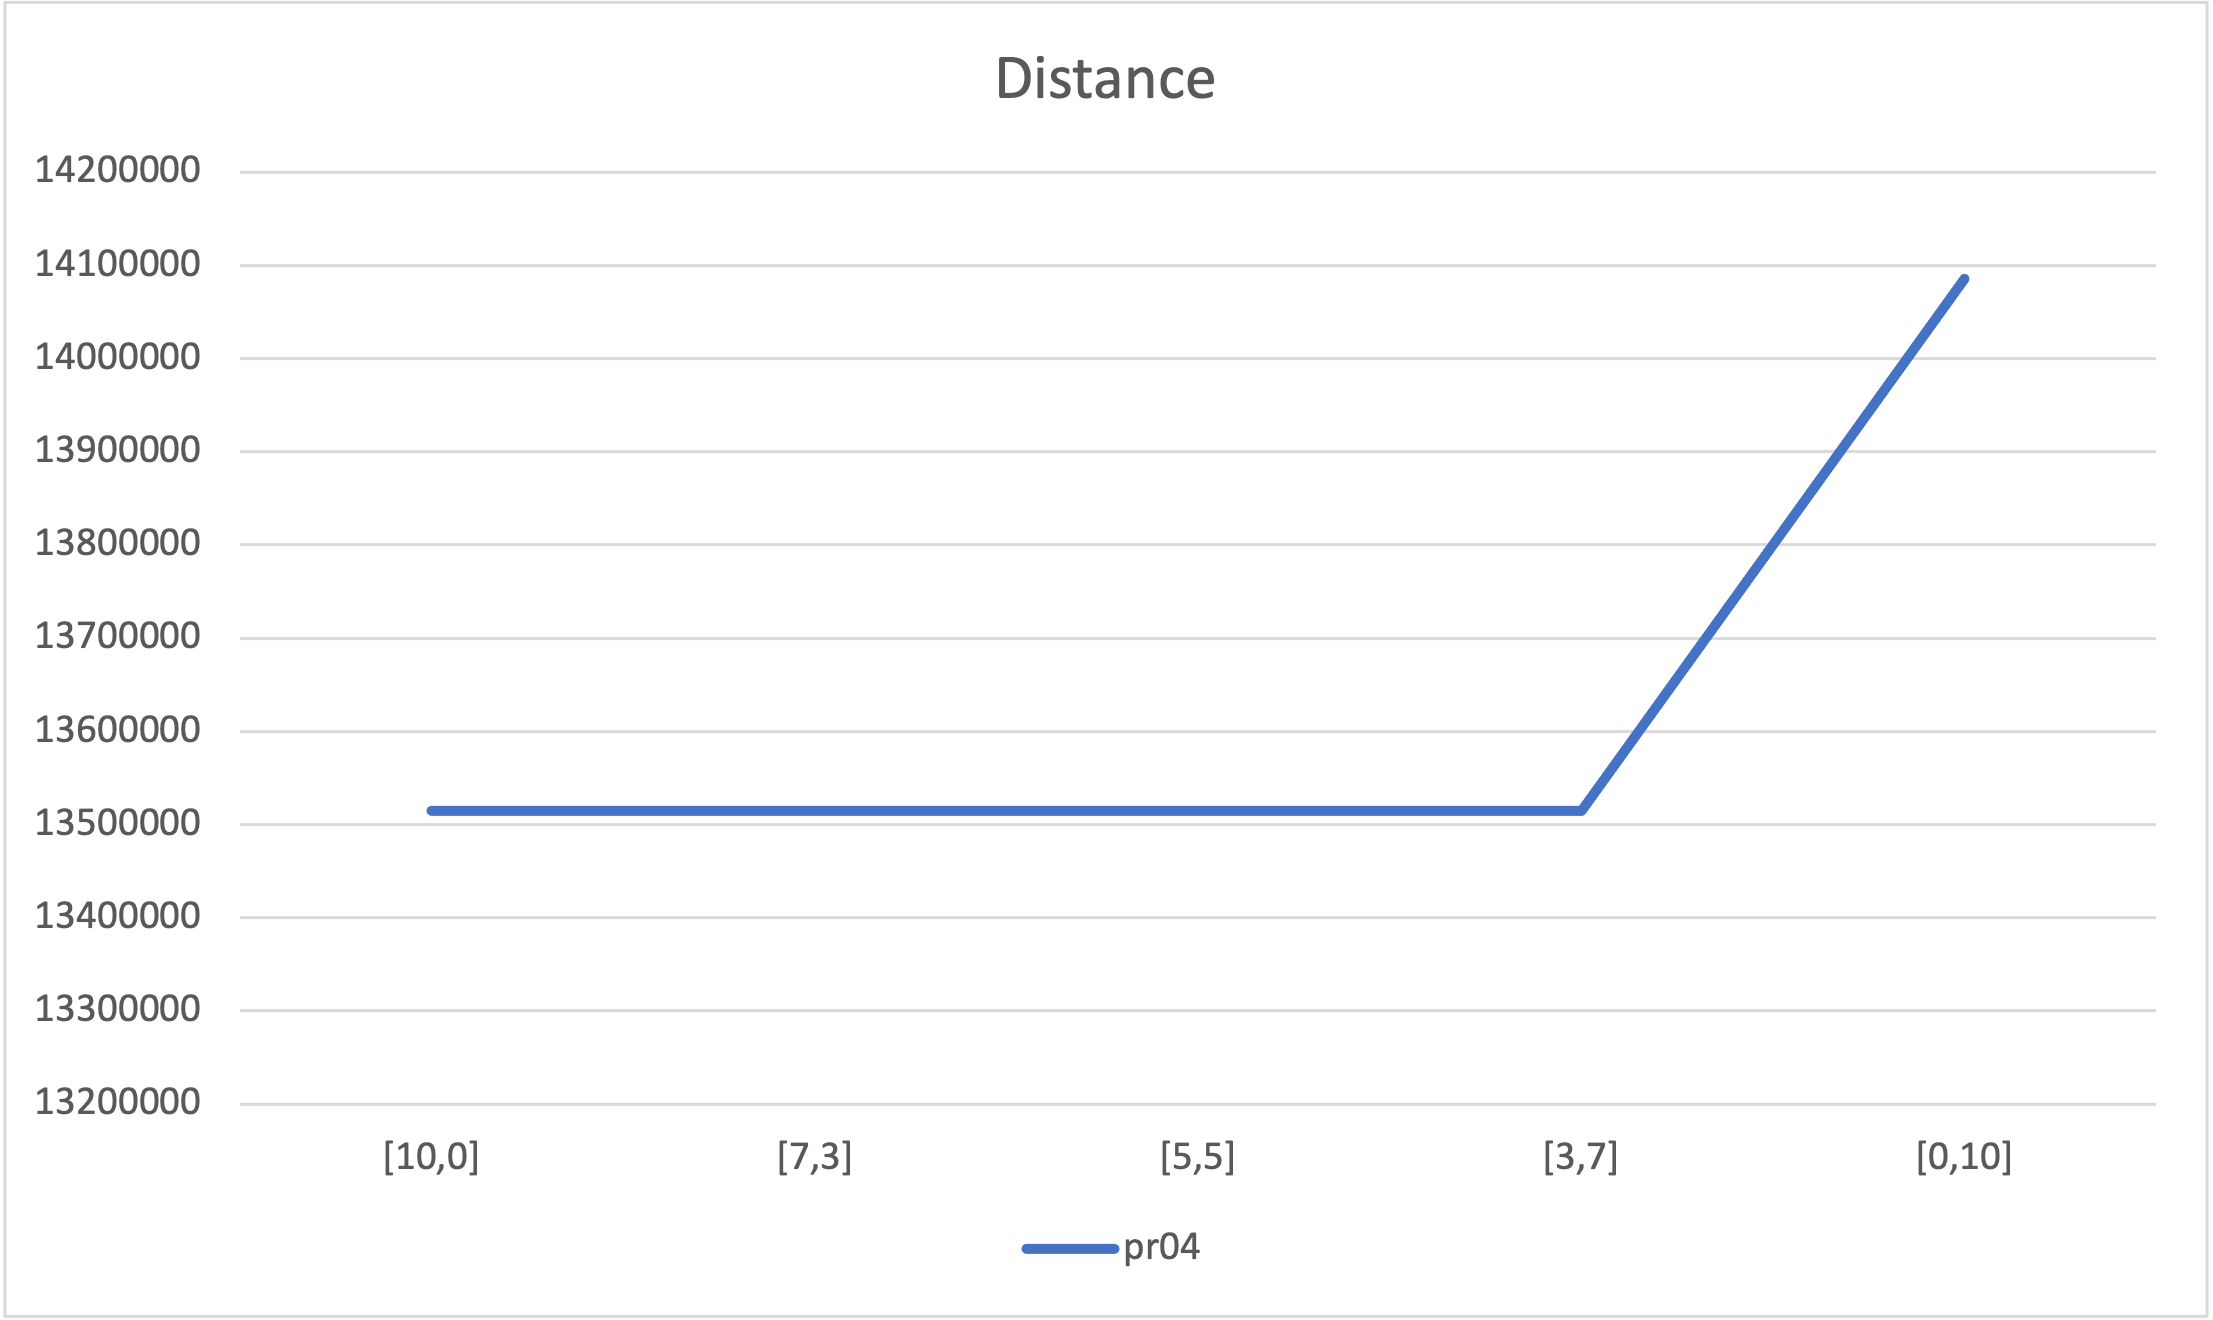
\includegraphics[height=0.25\textheight]{../graphs/pr04-distance.png}
    \caption{Distances graph for pr04.}
\end{figure}

\begin{figure}[H]
    \centering
    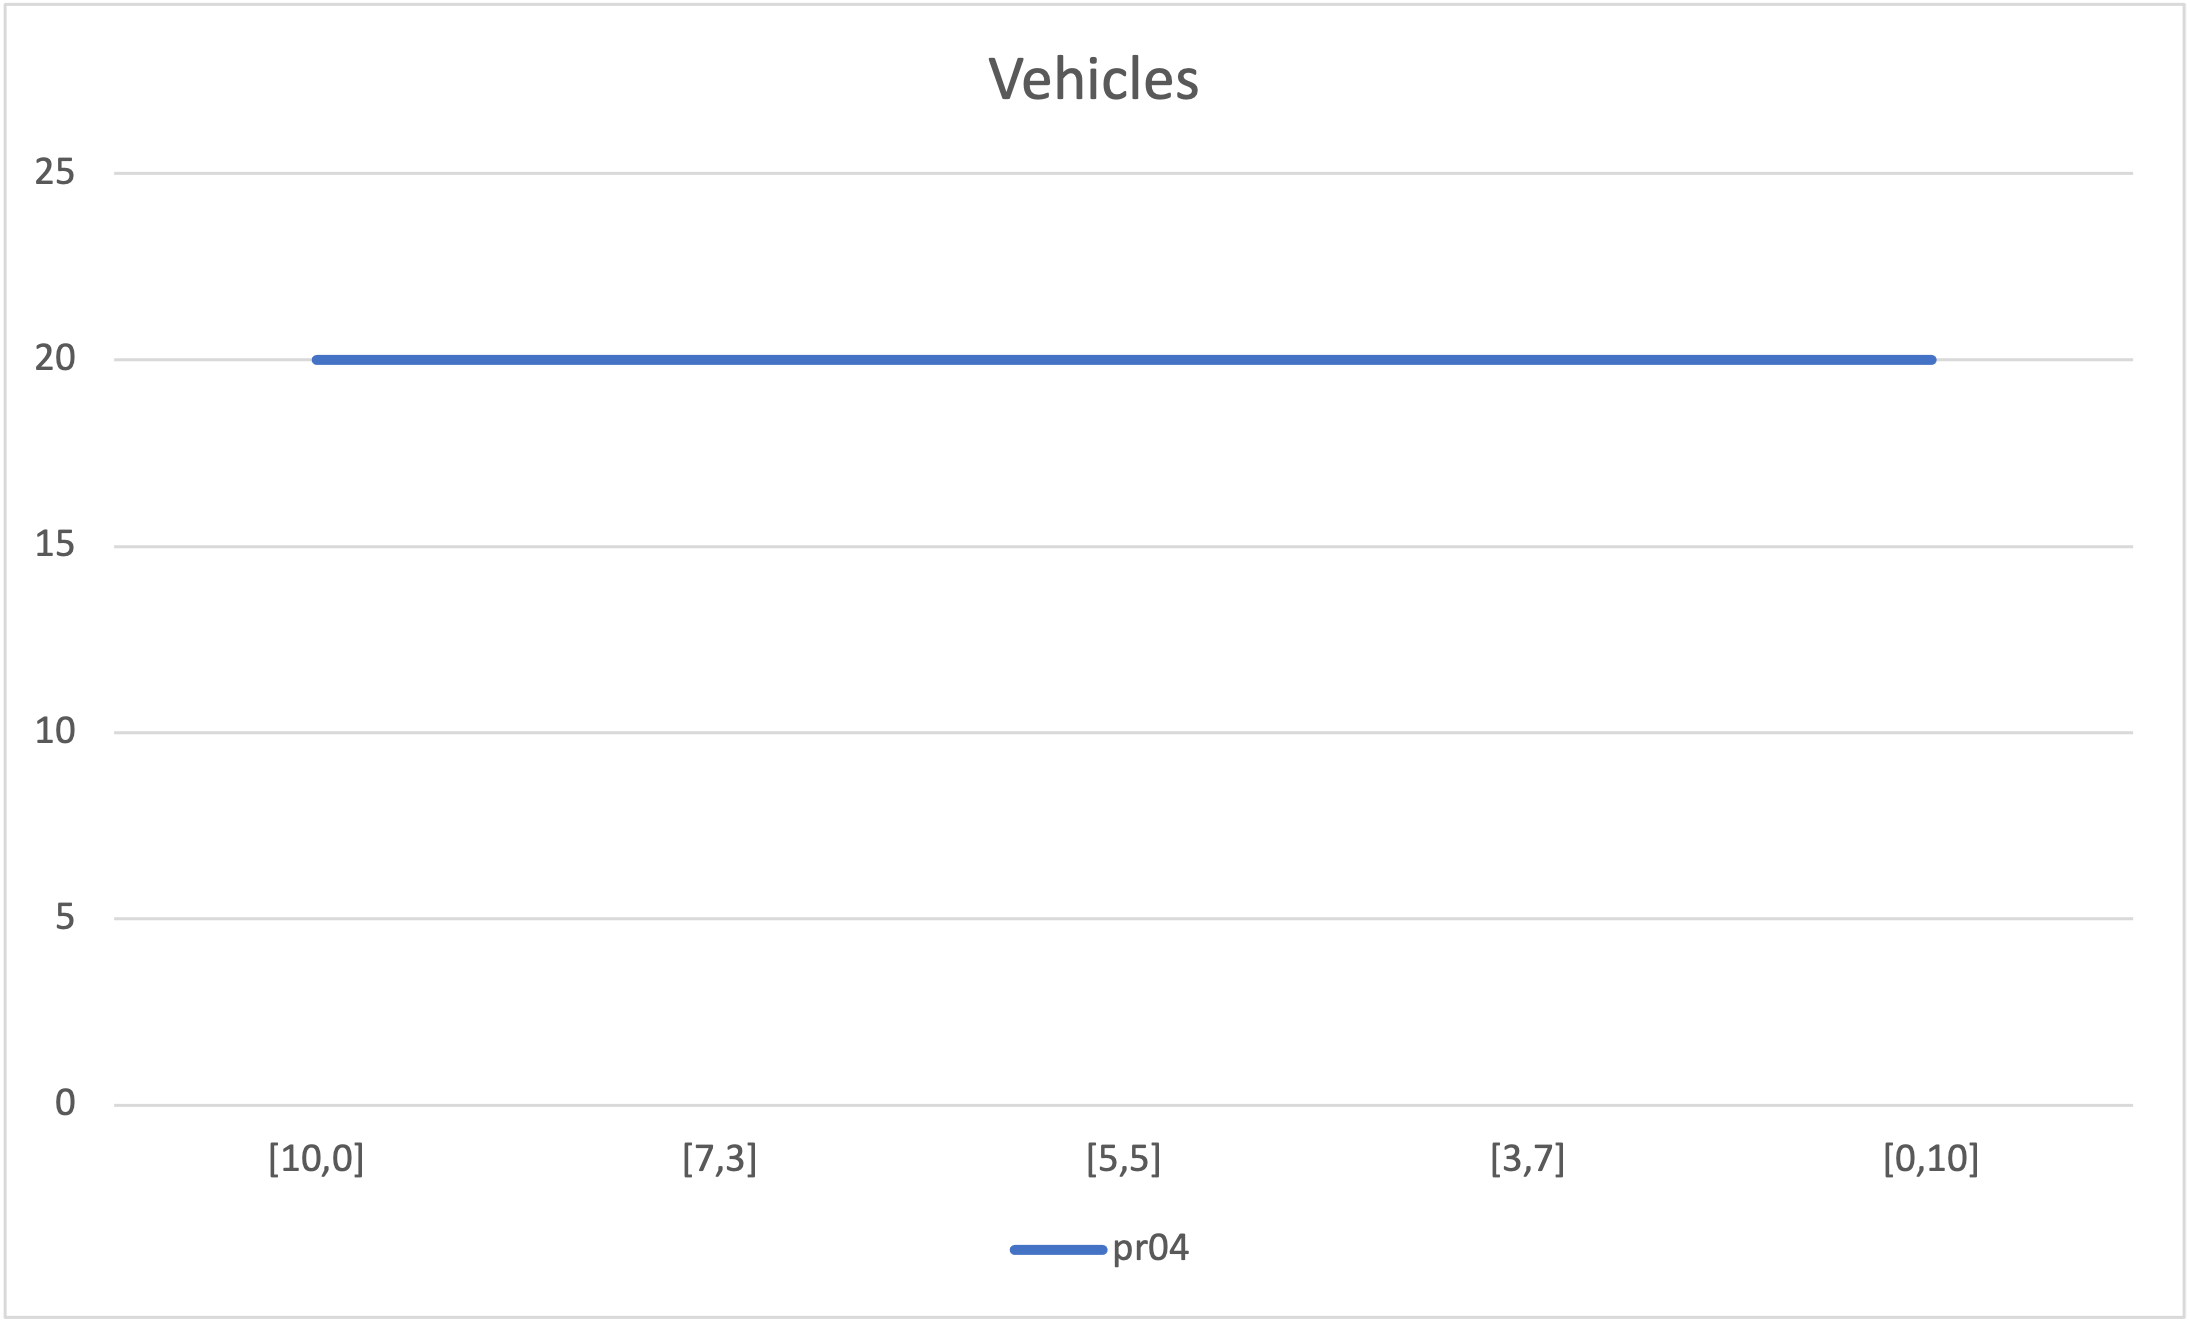
\includegraphics[height=0.25\textheight]{../graphs/pr04-vehicles.png}
    \caption{Vehicles used graph for pr04.}
\end{figure}

\newpage